\documentclass{beamer}

\mode<presentation> {
\usetheme{AnnArbor}
}

\usepackage{graphicx}
\graphicspath{{./figures/}}
\usepackage{caption}
\usepackage{subcaption}
\usepackage{hyperref}
\hypersetup{colorlinks=true}
\usepackage{amsmath}
\usepackage{amsthm}
%\usepackage[shortlabels]{enumitem}
\usepackage{biblatex}
\addbibresource{bibliography.bib}

\newcommand{\MDA}{\text{MDA}}
\newtheorem{proposition}{Proposition}

\title[Statistical Methods for Extremal Events]{Statistical Methods for Extremal Events}

\author{Victor Verma}
\institute[]
{
Prof. Yang Chen's Reading Group \\
Department of Statistics \\
University of Michigan
}
\date[2/23/23]{2/23/23}

\begin{document}

\begin{frame}
    \titlepage
\end{frame}

\begin{frame}{Today's Reading}
    \begin{itemize}
        \item Chapter 6 of \textit{Modelling Extremal Events} by Embrechts, Kl\"{u}ppelberg, and Mikosch (\cite{embrechts_et_al_1997})
    \end{itemize}
\end{frame}

%\begin{frame}{Outline}
%    \tableofcontents
%\end{frame}

\begin{frame}{Parameter Estimation for the GEV Distribution}
    Recall that a GEV (generalized extreme value) distribution $H_{\xi; \mu, \psi}$ satisfies
    \begin{align*}
        H_{\xi; \mu, \psi}(x) &= \exp\left\{-\left(1 + \xi\frac{x - \mu}{\psi}\right)^{-1 / \xi}\right\}, \quad 1 + \xi(x - \mu) / \psi > 0 \\
        &=
        \begin{cases}
            \Phi_{\alpha}\left(1 + \frac{x - \mu}{\alpha\psi}\right), & x > \mu - \psi\alpha, \ \xi = 1 / \alpha > 0 \\
            \Psi_{\alpha}\left(-\left(1 - \frac{x - \mu}{\alpha\psi}\right)\right), & x < \mu + \psi\alpha, \ \xi = -1 / \alpha < 0 \\
            \Lambda\left(\frac{x - \mu}{\psi}\right), & x \in \mathbb{R}, \ \xi = 0
        \end{cases}
    \end{align*}
    where
    \begin{align*}
        \text{(Fr\'{e}chet)} \quad \Phi_{\alpha}(x) &= \exp\left\{-x^{-\alpha}\right\}I_{(0, \infty)}(x) \\
        \text{(Weibull)} \quad \Psi_{\alpha}(x) &= \exp\{-(-x)^{\alpha}\}I_{(-\infty, 0)}(x) + I_{[0, \infty)}(x) \\
        \text{(Gumbel)} \quad \Lambda(x) &= \exp\left\{-e^{-x}\right\}
    \end{align*}
\end{frame}

\begin{frame}{Parameter Estimation for the GEV Distribution}
    \begin{itemize}
        \item $\xi \in \mathbb{R}$ is a shape parameter
        \item $\mu \in \mathbb{R}$ is a location parameter
        \item $\psi \in \mathbb{R}_+$ is a scale parameter
    \end{itemize}
    We write $H_{\xi; \mu, \psi}$ as $H_{\theta}$, where $\theta = (\xi, \mu, \psi)$. We also write $H_{\xi; 0, 1}$ as $H_{\xi}$.

    \smallskip

    Question: if $X_1, \ldots, X_n \overset{\text{iid}}{\sim} H_{\theta}$, how can we estimate $\theta$?
\end{frame}

\begin{frame}{Parameter Estimation for the GEV Distribution}
    $\theta$ can be estimated using maximum likelihood estimation.

    \medskip
    
    If $\xi \ne 0$, the log-likelihood is
    \begin{align*}
        \ell(\theta; \mathbf{X}) &= 
        -n\log\sigma \\
        &\quad - (1 + 1 / \xi)\sum_{i = 1}^n \log\left[1 + \xi\left(\frac{X_i - \mu}{\sigma}\right)\right] \\
        &\quad - \sum_{i = 1}^n \left[1 + \xi\left(\frac{X_i - \mu}{\sigma}\right)\right]^{-1 / \xi}
    \end{align*}
    when $1 + \xi(X_i - \mu) / \sigma > 0$ for $i = 1, \ldots, k$; it is $-\infty$ otherwise. If $\xi = 0$, the log-likelihood is
    \[
    \ell(\mu, \psi; \mathbf{X}) = -n\log\psi - \sum_{i = 1}^n \left(\frac{X_i - \mu}{\psi}\right) - \sum_{i = 1}^n \exp\left[-\left(\frac{X_i - \mu}{\psi}\right)\right]
    \]
\end{frame}

\begin{frame}{Parameter Estimation for the GEV Distribution}
    Numerical methods are required to compute the MLE in both cases.

    \medskip

    The MLE is efficient, consistent, and asymptotically normal in regular cases. A non-regular case occurs when the support of $H_{\theta}$ depends on $\theta$. In non-regular cases, the MLE may not have nice properties even if it can be estimated.

    \medskip

    It is known that the MLE has nice properties when $\xi > -1 / 2$ and that it doesn't when $\xi \le -1 / 2$. If the support of $H_{\theta}$ is unbounded above, then $\xi \ge 0 > -1 / 2$.
\end{frame}

\begin{frame}{Estimating Under MDA Conditions}
    \begin{definition}
        We say that the rv $X$ (the df $F$ of $X$, the distribution of $X$) belongs to the \textbf{maximum domain of attraction} of the extreme value distribution $H_{\xi; \mu, \psi}$ if there exist constants $c_n > 0, d_n \in \mathbb{R}$ such that $c_n^{-1}(M_n - d_n) \xrightarrow{d} H_{\xi; \mu, \psi}$. We write $X \in \MDA(H_{\xi; \mu, \psi})$ or $F \in \MDA(H_{\xi; \mu, \psi})$. $c_n$ and $d_n$ are called \textbf{norming constants}.
    \end{definition}
    Some facts about MDAs:
    \begin{itemize}
        \item $F \in \MDA(H_{\xi; \mu, \psi})$ with norming constants $c_n > 0, d_n \in \mathbb{R}$ iff $\lim_{n \to \infty} n\bar{F}(c_n x + d_n) = -\log H_{\xi; \mu, \psi}(x)$ for all $x \in \mathbb{R}$.
        \item $\MDA(H_{\xi; \mu, \psi}) = \MDA(H_{\xi; 0, 1}) = \MDA(H_{\xi})$.
        \item $F \in \MDA(\Phi_{\alpha})$ iff $\bar{F} \in \mathcal{R}_{-\alpha}$, i.e., $\bar{F}$ is \textbf{regularly varying}; $\lim_{t \to \infty} \bar{F}(t x) / \bar{F}(t) = x^{-\alpha}$ for all $x > 0$.
    \end{itemize}
\end{frame}

\begin{frame}{Estimating Under MDA Conditions}
    Question: if $X_1, \ldots, X_n \overset{\text{iid}}{\sim} F \in \MDA(H_{\xi})$, how can we estimate $\xi$?

    \medskip

    An example showing how this differs from the previous question:

    \medskip
    
    Let $\Phi_{\alpha}(x) = \exp\{-x^{-\alpha}\}, x > 0$ is the df of the standard $\alpha$-Fr\'{e}chet distribution. \\
    If $X_1, \ldots, X_n \overset{iid}{\sim} F = \Phi_{\alpha}$, then
    \[
    \bar{F}(x) = 1 - \exp\{-x^{-\alpha}\}, x > 0.
    \]
    If $X_1, \ldots, X_n \overset{iid}{\sim} F \in \MDA(\Phi_{\alpha})$, then $\bar{F} \in \mathcal{R}_{-\alpha}$, so
    \[
    \bar{F}(x) = x^{-\alpha}L(x), x > 0,
    \]
    where $L$ is \textbf{slowly varying}, i.e., $L \in \mathcal{R}_0$.
\end{frame}

\begin{frame}{Estimating Under MDA Conditions}
    Since $X_1, \ldots, X_n \overset{\text{iid}}{\sim} F \in \MDA(H_{\xi})$, for $u = c_n x + d_n$,
    \begin{align*}
        n\bar{F}(u) &\approx -\log H_{\xi}(x) \\
        &\approx \left(1 + \xi\frac{u - d_n}{c_n}\right)^{-1 / \xi} \\
        \bar{F}(u) &\approx \frac{1}{n}\left(1 + \xi\frac{u - d_n}{c_n}\right)^{-1 / \xi}.
    \end{align*}
    With estimates $\hat{\xi}$, $\hat{c_n}$, and $\hat{d_n}$, we could estimate $\bar{F}(u)$ as
    \[
    \widehat{\bar{F}(u)} = \frac{1}{n}\left(1 + \hat{\xi}\frac{u - \hat{d_n}}{\hat{c_n}}\right)^{-1 / \hat{\xi}}.
    \]
\end{frame}

\begin{frame}{Estimating Under MDA Conditions}
    $F \in \MDA(H_{\xi})$ is a tail property (e.g., $F \in \MDA(\Phi_{\alpha}) \implies \bar{F} \in \mathcal{R}_{-\alpha}$), so $\hat{\xi}$ can be computed from the $k$ largest order statistics $X_{k, n} \le \ldots \le X_{1, n}$.

    \medskip

    Typical conditions imposed on $k = k(n)$:
    \begin{itemize}
        \item $\lim_{n \to \infty} k(n) = \infty$
        \item $\lim_{n \to \infty} \frac{n}{k(n)} = \infty$
    \end{itemize}
\end{frame}

\begin{frame}{The Pickands Estimator of $\xi$}
    The \textbf{Pickands estimator} of $\xi$ is defined as
    \[
    \hat{\xi}_{k, n}^{(P)} = \frac{1}{\log 2}\log\frac{X_{k, n} - X_{2 k, n}}{X_{2 k, n} - X_{4 k, n}}
    \]
\end{frame}

\begin{frame}{The Pickands Estimator of $\xi$}
    \begin{proposition}
        Suppose $\{X_n\}$ is an iid sequence with df $F \in \MDA(H_{\xi})$, $\xi \in \mathbb{R}$. Let $\hat{\xi}^{(P)} = \hat{\xi}_{k, n}^{(P)}$ be the Pickands estimator.
        \begin{enumerate}
            \item[(a)] (Weak consistency) If $k \to \infty$, $k / n \to 0$ for $n \to \infty$, then $\hat{\xi}^{(P)} \xrightarrow{P} \xi, \quad n \to \infty$.
            \item[(b)] (Strong consistency) If $k / n \to 0$, $k / \log\log n \to \infty$ for $n \to \infty$, then 
            $\hat{\xi}^{(P)} \xrightarrow{a.s.} \xi, \quad n \to \infty$.
            \item[(c)] (Asymptotic normality) Under further conditions on $k$ and $F$,
            \[
            \sqrt{k}(\hat{\xi} - \xi) \xrightarrow{d} N(0, v(\xi)), \quad n \to \infty,
            \]
            where
            \[
            v(\xi) = \frac{\xi^2(2^{2\xi + 1} + 1)}{(2(2^{\xi} - 1)\log 2)^2}.
            \]
        \end{enumerate}
    \end{proposition}    
\end{frame}

\begin{frame}{Q-Q Plots}
    The motivating question: \textit{Find a df F which is a good model for the iid data $X, X_1, \ldots, X_n$}.

    \medskip

    Suppose that $X_1, \ldots, X_n \sim G(x) = F\left(\frac{x - \mu}{\sigma}\right)$ for some continuous df $F$, some $\mu \in \mathbb{R}$, and some $\sigma > 0$. Let $X_{n, n} \le \ldots \le X_{1, n}$ be the order statistics of the sample and let $G_n$ be the empirical df.

    \medskip

    Using the probability integral transform, $U_i = G(X_i) \sim \text{Uniform}(0, 1)$. Moreover,
    \[
    (G(X_{k, n})_{k = 1, \ldots, n} \overset{d}{=} (U_{k, n})_{k = 1, \ldots, n}.
    \]
    Since $U_{k, n}$ has pdf $\frac{n!}{(n - k)!(k - 1)!}u^{n - k}(1 - u)^{k - 1}I_{(0, 1)}(u)$ \cite{casella_and_berger_2002},
    \[
    E[G(X_{k, n})] = E(U_{k, n}) = \frac{n - k + 1}{n + 1}.
    \]
\end{frame}

\begin{frame}{Q-Q Plots}
    Thus, for large $n$,
    \[
    X_{k, n} = G_n^{\leftarrow}\left(\frac{n - k + 1}{n}\right) \approx G^{\leftarrow}\left(\frac{n - k + 1}{n + 1}\right) = \sigma F^{\leftarrow}\left(\frac{n - k + 1}{n + 1}\right) + \mu,
    \]
    so the graph
    \[
    \left\{\left(F^{\leftarrow}\left(\frac{n - k + 1}{n + 1}\right), X_{k, n}\right) : k = 1, \ldots, n\right\}
    \]
    should look linear.

    \smallskip

    This graph is a called a \textbf{Q-Q (quantile-quantile)} plot.
\end{frame}

\begin{frame}{Q-Q Plots}
    \begin{figure}
        \centering
        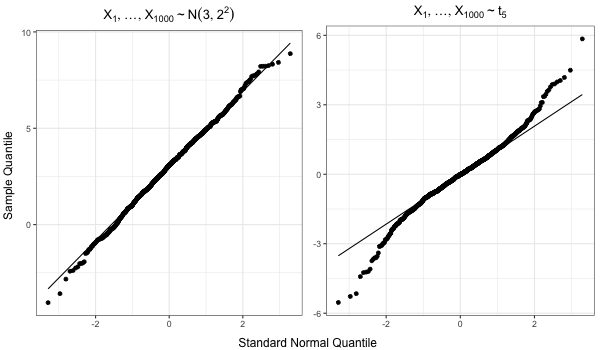
\includegraphics[scale=0.5]{qq_plots.png}
        \caption{Example Q-Q plots.}
        \label{fig:qq_plots}
    \end{figure}
\end{frame}

\begin{frame}{Q-Q Plots}
    Things we can do with Q-Q plots:
    \begin{enumerate}
        \item Check whether a proposed distribution for $X, X_1, \ldots, X_n$ is plausible
        \item Check for outliers
        \item Estimate location and scale parameters
        \item Compare shapes of distributions
    \end{enumerate}
\end{frame}

\begin{frame}{Q-Q Plots}
    The GEV family isn't a location-scale family, but it has location-scale subfamilies. A strategy for making a Q-Q plot in the GEV case:
    \begin{enumerate}
        \item Compute an estimate $\hat{\xi}$ of $\xi$ (more on this later).
        \item Make a Q-Q plot with $X_1, \ldots, X_n$ and $H_{\hat{\xi}; 0, 1}$
    \end{enumerate}
    From the Q-Q plot, estimates $\hat{\mu}$ of $\mu$ and $\hat{\psi}$ of $\psi$ can be computed. $\hat{\xi}$, $\hat{\mu}$, and $\hat{\psi}$ can be used as initial values in a numerical procedure for obtaining more accurate estimates.
\end{frame}

\begin{frame}{Threshold Excesses}
    Let $X, X_1, X_2, \ldots$ be iid rvs with common df $F$. Two ways of thinking about extremes:
    \begin{itemize}
        \item The maximum $\vee_{i = 1}^n X_i$
        \item The \textbf{threshold excess} $X - u$ when $X > u$, where $u$ is a high threshold
    \end{itemize}
    The block maximum approach uses maxima. It can waste useful data if some blocks contain multiple extreme values.

    \begin{definition}
        Let $X$ be a rv with df $F$ and right endpoint $x_F$. For a fixed $u < x_F$,
        \[
        F_u(x) = P(X - u \le x | X > u), \ x \ge 0,
        \]
        is the \textbf{excess df} of the rv $X$ (of the df $F$) over the threshold $u$.
    \end{definition}
\end{frame}

\begin{frame}{Threshold Excesses}
    \begin{proposition} % Theorem 4.1 in Coles
        Let $X, X_1, X_2, \ldots$ be iid rvs with common df $F$ and let $M_n = \max_{i = 1, \ldots, n} X_i$. Suppose that $F$ is in the MDA of a GEV distribution; for large $n$, $P(M_n \le z) \approx G(z)$, where
        \[
        G(z) = \exp\left\{-\left[1 + \xi\left(\frac{z - \mu}{\sigma}\right)\right]^{-1 / \xi}\right\}
        \]
        for some $\mu$, positive $\sigma$, and $\xi$. Then for large enough $u$,
        \[
        F_u(y) \approx 1 - \left(1 + \frac{\xi y}{\tilde{\sigma}}\right)^{-1 / \xi}
        \]
        on $\{y : y > 0, 1 + \xi y / \tilde{\sigma} > 0\}$, where $\tilde{\sigma} = \sigma + \xi(u - \mu)$.
    \end{proposition}
\end{frame}

\begin{frame}{The Generalized Pareto Distribution}
    A distribution with df of the form
    \[
    1 - \left(1 + \frac{\xi y}{\sigma}\right)^{-1 / \xi}
    \]
    supported on $\{y : y > 0, 1 + \xi y / \sigma > 0\}$, with $\xi \in \mathbb{R}$ and $\sigma > 0$, is called a \textbf{generalized Pareto (GP) distribution}. When $\xi = 0$, this is defined by continuity as $1 - e^{-y / \sigma}$, the df of the exponential distribution with mean $\sigma$.
\end{frame}

\begin{frame}{The Mean Excess Function}
    \begin{definition}
        Let $X$ be a rv with right endpoint $x_F$; then
        \[
        e(u) = E(X - u | X > u), 0 \le u < x_F,
        \]
        is called the \textbf{mean excess function} of $X$.
    \end{definition}
\end{frame}

\begin{frame}{The Mean Excess Function}
    Suppose that $X$ is a positive rv with df $F$ and finite expectation. Then
    \begin{align*}
        e(u) &= \frac{1}{\bar{F}(u)}\int_u^{x_F} (x - u)\,dF(x) \\
        &= \frac{1}{\bar{F}(u)}\int_u^{x_F} \bar{F}(x)\,dx, \quad 0 < u < x_F.
    \end{align*}
    If $F$ is continuous,
    \[
    \bar{F}(x) = \frac{e(0)}{e(x)}\exp\left\{-\int_0^x \frac{1}{e(u)}\,du\right\}.
    \]
    This implies that a continuous df is uniquely determined by its mean excess function.
\end{frame}

\begin{frame}{The Mean Excess Function}
    \begin{figure}
        \centering
        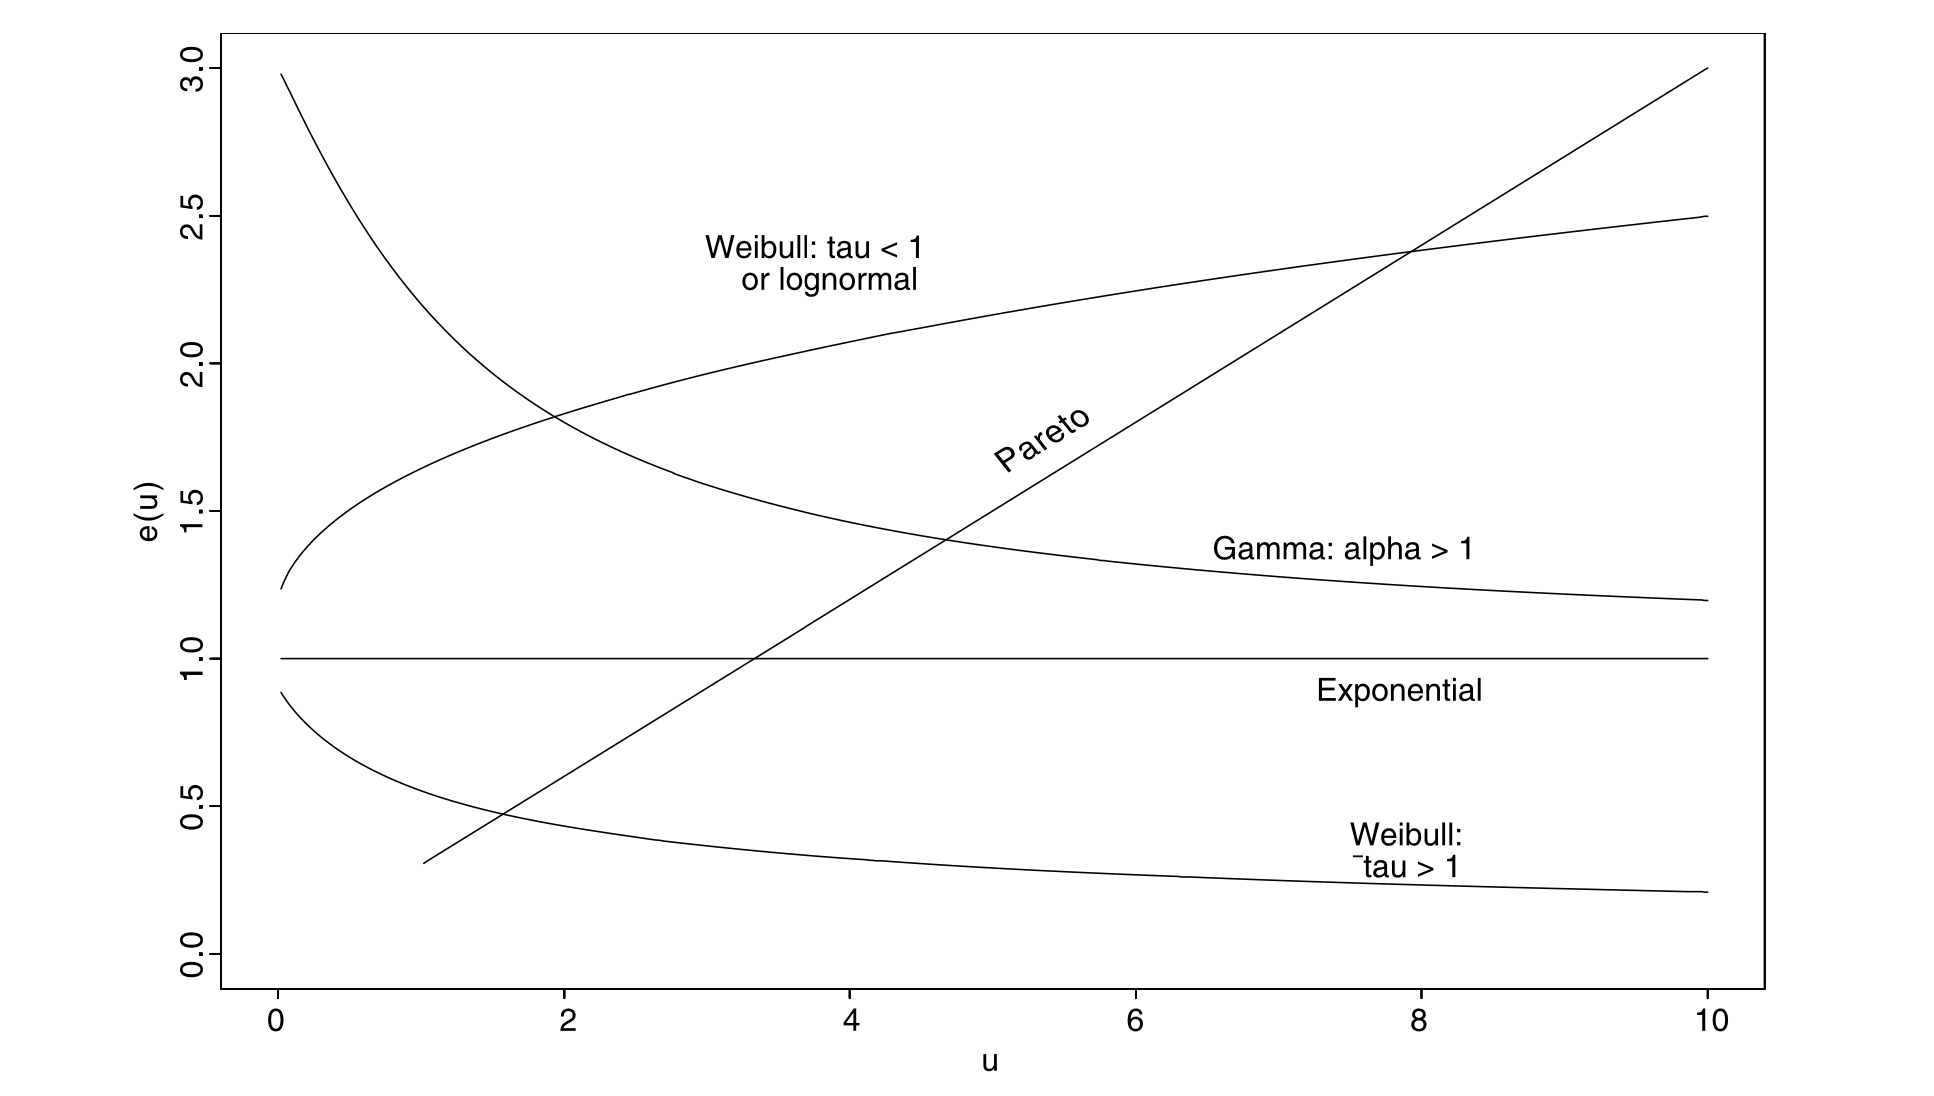
\includegraphics[scale=0.32]{mean_excess_functions.png}
        \caption{Some mean excess functions (source: \cite{embrechts_et_al_1997})}
        \label{fig:mean_excess_functions}
    \end{figure}
\end{frame}

\begin{frame}{The Mean Excess Function}
    \begin{proposition}
        Suppose $X$ has GPD with parameters $\xi < 1$ and $\sigma$. Then for $u < x_F$,
        \[
        e(u) = E(X - u | X > u) = \frac{\sigma + \xi u}{1 - \xi}, \ \sigma + \xi u > 0.
        \]
    \end{proposition}
\end{frame}

\begin{frame}{The Mean Excess Function}
    \begin{definition}
        Let $X_1, \ldots, X_n \overset{\text{iid}}{\sim} F$, let $F_n$ be the empirical df, and let $\triangle_n(u) = \{i : i = 1, \ldots, n, \ X_i > u\}$. The \textbf{empirical mean excess function} $e_n$ is defined by
        \[
        e_n(u) = \frac{1}{\#\triangle_n(u)}\sum_{i \in \delta_n(u)} (X_i - u), \ u \ge 0,
        \]
        with the convention that $0 / 0 = 0$.
    \end{definition}
\end{frame}

\begin{frame}{Mean Residual Life Plots}
    Suppose that $F_u$ can be modeled as a GPD for large $u$. How can these $u$ be identified?

    \smallskip

    One approach is to make a \textbf{mean residual life plot}. This is a plot of points of the form $(u, e_n(u))$. Let $\xi$ and $\sigma$ be the parameters of the approximating GPD. Then for large $u$,
    \[
    e_n(u) \approx e(u) \approx \frac{\sigma + \xi u}{1 - \xi}
    \]
    Suitable $u$ are those for which $(u, e_n(u))$ roughly fall along a line.

    \smallskip

    Mean residual life plots can be difficult to interpret, as the example on the next slide shows.
\end{frame}

\begin{frame}{Mean Residual Life Plots}
    \begin{figure}
        \centering
        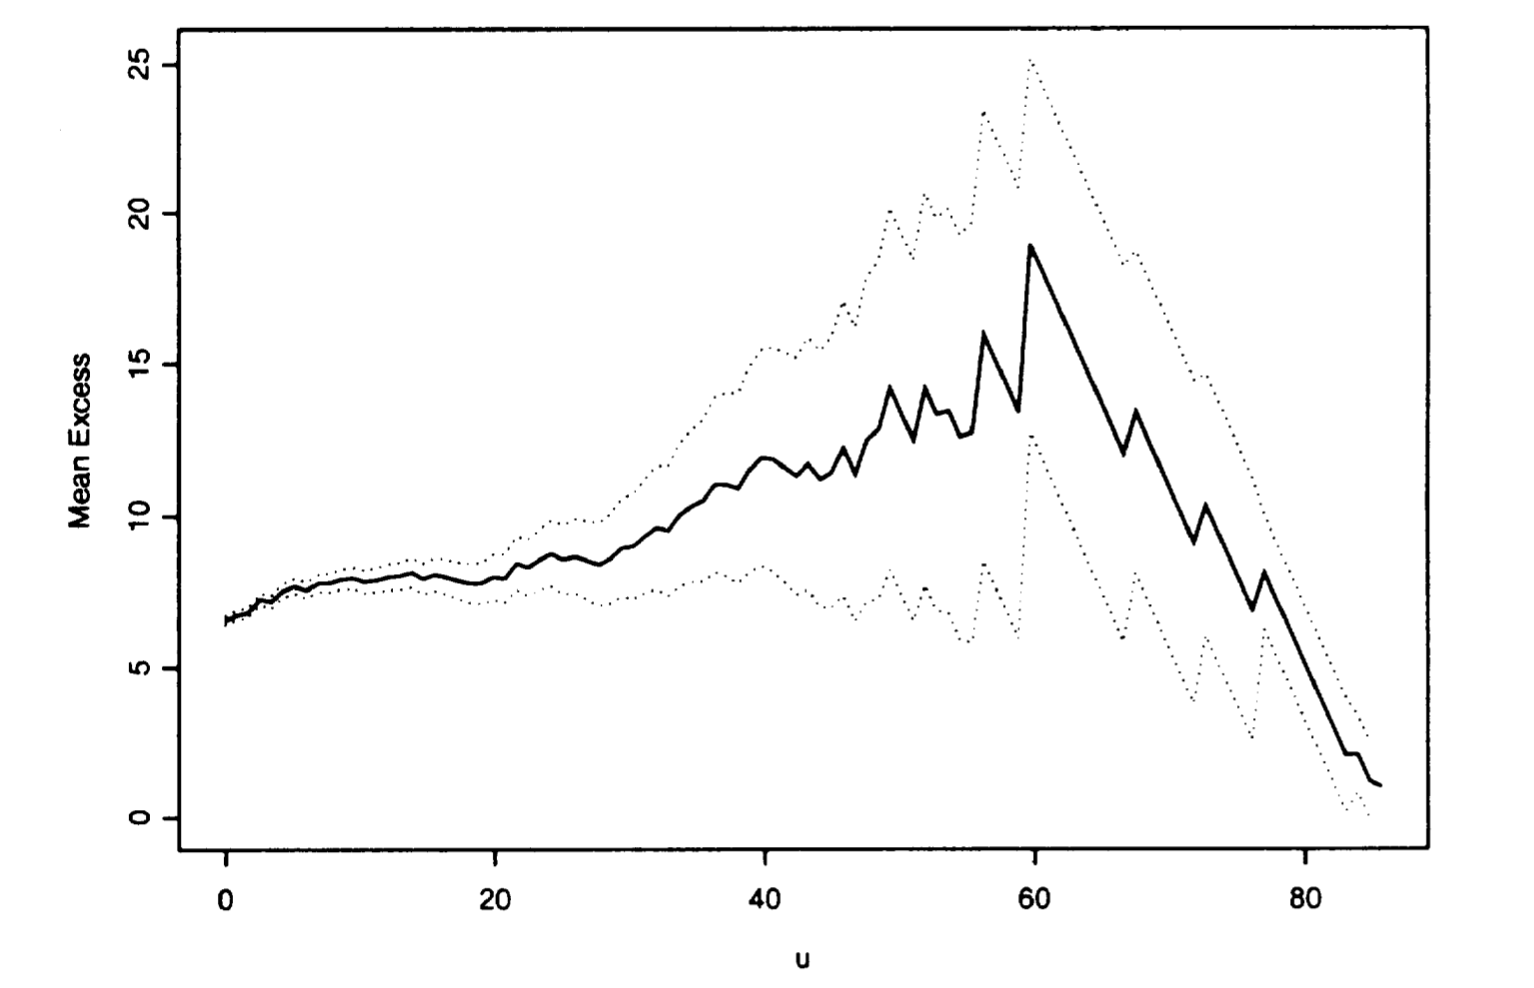
\includegraphics[scale=0.35]{mean_residual_life_plot.png}
        \caption{An example mean residual life plot (source: \cite{coles_2001}).}
        \label{fig:mean_residual_life_plot}
    \end{figure}
\end{frame}

\begin{frame}{GPD Parameter Estimation}
    A GPD is fit using maximum likelihood estimation. Suppose that there are $k$ excesses $Y_1, \ldots, Y_k$ of the selected threshold $u$. If $\xi \ne 0$, then the log-likelihood is
    \[
    \ell(\xi, \sigma) = -k\log\sigma - (1 + 1 / \xi)\sum_{i = 1}^k \log(1 + \xi Y_i / \sigma)
    \]
    when $1 + \xi Y_i / \sigma > 0$ for $i = 1, \ldots, k$; otherwise, $\ell(\xi, \sigma) = -\infty$. If $\xi = 0$, the log-likelihood is
    \[
    \ell(\sigma) = -k\log\sigma - \frac{1}{\sigma}\sum_{i = 1}^k Y_i.
    \]
    Numerical methods are required to find the MLEs.
\end{frame}

\begin{frame}{References}
    \nocite{*}
    \printbibliography
\end{frame}

\end{document}